%!TEX root = ../dissertation.tex

% =====================================================================
%  CHAPTER 4 — METHODOLOGY   (DRAFT v1, full prose)
% ---------------------------------------------------------------------
%  Notation (defined in dissertation.tex, i-CIR-aligned):
%   \qv q^v query image | \qt q^t query text | \qc c target caption
%   \DB X database | \xdb x a db image | \encv \enct encoders
%   \simop sim | \clamp clamp | \sv \st \sc the three scores
%  Rule: this chapter says WHAT and WHY. All numbers live in Chapter 5.
%  HIGHLIGHT markers = figures to insert or facts to verify.
% =====================================================================

\chapter{Methodology}\label{chapt:method}

This chapter presents the proposed approach to zero-shot instance-level
composed image retrieval. The central idea is to add a third retrieval
modality: in addition to the reference image and the modification text, a frozen
multimodal large language model generates a \emph{target caption} -- a short
description of the image the user has in mind -- and the three resulting
similarities are combined by a late-fusion product. The chapter is organised as
follows.
Section~\ref{sect:method_problem} formalises the composed image retrieval task
and fixes the notation used throughout the thesis.
Section~\ref{sect:method_eval} defines the evaluation protocol and metrics.
Section~\ref{sect:method_overview} gives an overview of the proposed retrieval
pipeline.
Section~\ref{sect:method_backbones} describes the vision--language backbones
used to embed the data.
Section~\ref{sect:method_basic} recalls the \textsc{Basic} baseline that this
work builds upon.
Section~\ref{sect:method_caption} introduces the target-caption generation
step, the central contribution.
Section~\ref{sect:method_fusion} presents the triplet late-fusion scoring
function.
Section~\ref{sect:method_impl} reports the implementation details.

% =====================================================================
\section{Problem Formulation and Notation}\label{sect:method_problem}
% =====================================================================

\paragraph{Composed image retrieval.}
A composed image retrieval query is a pair $q = (\qv, \qt)$, where $\qv$ is a
reference \emph{query image} and $\qt$ is a short \emph{query text} that
specifies how the desired result should differ from $\qv$. Given a database of
images $\DB = \{\xdb_1, \dots, \xdb_N\}$, the goal is to produce a ranking of
$\DB$ that places the image the user intends -- the result of applying the
modification $\qt$ to the instance shown in $\qv$ -- as close to the top as
possible. We denote by $\encv$ the visual encoder of a frozen vision--language
model and by $\enct$ its textual encoder; both map their input to an
$\ell_2$-normalised vector in a shared $d$-dimensional space, and similarity is
measured by the cosine similarity $\simop$ of Equation~\eqref{eq:cosine}.

\paragraph{Instance-level relevance.}
This thesis adopts the instance-level protocol of the i-CIR
benchmark~\cite{psomas2025icir}. Unlike category-level CIR, where any image of
the right category is acceptable, here a database image is \emph{relevant} to a
query only if it depicts the same object \emph{instance} as $\qv$, modified as
$\qt$ requests. Ground truth is defined at this instance granularity, so the
positive set of a query is typically small and specific. The benchmark
deliberately surrounds each query with \emph{hard negatives}, which we group
into three types following the dataset design: \emph{visual} hard negatives
(the same or a visually similar instance that does \emph{not} satisfy the
modification), \emph{textual} hard negatives (images that satisfy the
modification text but show a \emph{different} instance), and \emph{composed}
hard negatives (the correct instance under a \emph{different} modification).
This structure is what makes instance-level CIR difficult: a method must
jointly preserve the visual identity of the instance \emph{and} apply the
precise change demanded by the text, since collapsing onto either modality
alone aligns the method with one of the hard-negative types.

\paragraph{Scale.}
% HIGHLIGHT: verify these counts against the i-CIR data card.
The full benchmark comprises $1{,}883$ queries and $N = 752{,}092$ database
images. For development we use a fixed $20\%$ instance subset ($400$ queries and
$N = 143{,}769$ database images; see Section~\ref{sect:method_impl}), on which
the ablation studies of Chapter~\ref{chapt:results} are conducted.

\paragraph{Zero-shot assumption.}
We operate strictly in the \emph{zero-shot} regime: no component of the system
is trained or fine-tuned on i-CIR. All encoders $\encv, \enct$ are
off-the-shelf, frozen vision--language models, the caption generator is a
frozen MLLM, and every fusion and post-processing step is training-free. We
adopt this setting both because the benchmark is intended for evaluation rather
than large-scale training and because it isolates the contribution of the
proposed retrieval signal from any benefit of supervision. The justification
for preferring zero-shot over a trained fusion model is given here, at the point
where the assumption is introduced, rather than deferred to the experiments.

% =====================================================================
\section{Evaluation Protocol and Metrics}\label{sect:method_eval}
% =====================================================================

\paragraph{Ranking protocol.}
Each query is evaluated by ranking the database (or, equivalently, its
instance pool) by decreasing fused similarity and comparing the ranking against
the query's relevant set, consistent with the i-CIR
protocol~\cite{psomas2025icir}.

\paragraph{Average precision.}
The primary quality measure is the average precision of the ranking, computed in
the trapezoidal (Oxford-style) form used by the benchmark and classical
instance retrieval~\cite{philbin2007oxford}. Writing the precision--recall
curve as the sequence of points $(r_0, p_0), (r_1, p_1), \dots$ obtained by
sweeping the rank threshold, the trapezoidal average precision integrates
precision over recall as
\begin{equation}\label{eq:ap}
    \mathrm{AP} = \sum_{i \geq 1} (r_i - r_{i-1})\,
    \frac{p_i + p_{i-1}}{2},
\end{equation}
i.e. the area under the precision--recall curve approximated by trapezoids
between successive recall levels.

\paragraph{Macro- vs.\ micro-averaging.}
% HIGHLIGHT: confirm this matches the paper's macro/micro definition exactly.
Because the number of queries per instance is uneven, we distinguish two ways of
aggregating AP. The \emph{micro}-averaged mAP (denoted \textsc{mAP}) is the mean
of AP over \emph{all queries}, giving every query equal weight. The
\emph{macro}-averaged mAP (denoted \textsc{mmAP}) first averages AP over the
queries belonging to each \emph{instance} and then averages across instances,
giving every instance equal weight regardless of how many queries it has.
Following the i-CIR benchmark, \textbf{macro-mAP is the primary metric}; it is
the headline number in all tables unless stated otherwise.

\paragraph{Auxiliary metrics.}
We additionally report rank-cutoff metrics: $\mathrm{Recall}@k$ (the fraction
of relevant items retrieved within the top-$k$, for $k \in \{10, 100\}$) and
$\mathrm{Hit}@k$ (whether at least one relevant item appears in the top-$k$,
for $k \in \{1, 10\}$). These characterise the top of the ranking, which is
what a user sees first.

% =====================================================================
\section{Pipeline Overview}\label{sect:method_overview}
% =====================================================================

Figure~\ref{fig:pipeline} summarises the proposed pipeline. The system has three
parallel branches that each produce a similarity between the query and a
candidate database image $\xdb$:
\begin{enumerate}
  \item the \emph{image branch} encodes the reference image $\qv$ with $\encv$
        and compares it to the encoded candidate, giving
        $\sv = \simop(\encv(\qv), \encv(\xdb))$;
  \item the \emph{text branch} encodes the modification text $\qt$ with $\enct$
        and compares it to the candidate, giving
        $\st = \simop(\enct(\qt), \encv(\xdb))$;
  \item the \emph{caption branch}, the contribution of this thesis, generates a
        target caption $\qc$ with a frozen MLLM, encodes it with $\enct$, and
        compares it to the candidate, giving
        $\sc = \simop(\enct(\qc), \encv(\xdb))$.
\end{enumerate}
The three scores are combined by the late-fusion product of
Section~\ref{sect:method_fusion} into a single score per candidate, and the
database is ranked by this fused score. Two properties are worth emphasising.
First, \emph{all encoders are frozen and off-the-shelf}: the only learning that
ever occurred is the original vision--language and MLLM pretraining. Second, the
caption branch is purely \emph{additive} -- it supplies a strong text-side query
without removing the visual signal from the image branch, which is what allows
the fusion to respect instance identity while applying the modification.

\begin{figure}[t]
\centering
\resizebox{\textwidth}{!}{% Pipeline overview — three-branch CIR method (TikZ/PGF)
%
% Add to dissertation.tex preamble:
%   \usepackage{tikz}
%   \usetikzlibrary{arrows.meta,shapes.geometric,positioning,calc,backgrounds}
%
% Usage in methodology.tex:
%   \begin{figure}[t]\centering
%     \resizebox{\textwidth}{!}{% Pipeline overview — three-branch CIR method (TikZ/PGF)
%
% Add to dissertation.tex preamble:
%   \usepackage{tikz}
%   \usetikzlibrary{arrows.meta,shapes.geometric,positioning,calc,backgrounds}
%
% Usage in methodology.tex:
%   \begin{figure}[t]\centering
%     \resizebox{\textwidth}{!}{% Pipeline overview — three-branch CIR method (TikZ/PGF)
%
% Add to dissertation.tex preamble:
%   \usepackage{tikz}
%   \usetikzlibrary{arrows.meta,shapes.geometric,positioning,calc,backgrounds}
%
% Usage in methodology.tex:
%   \begin{figure}[t]\centering
%     \resizebox{\textwidth}{!}{\input{figures/pipeline_overview}}
%     \caption{...}\label{fig:pipeline}
%   \end{figure}

\begin{tikzpicture}[
  >=Stealth, line cap=round, line join=round,
  font=\small,
  % ── node styles ───────────────────────────────────────────────────────
  enc/.style      = {draw=#1!65!black, fill=#1!10, rounded corners=3pt,
                      minimum width=1.85cm, minimum height=0.60cm,
                      align=center, inner sep=3pt},
  enc/.default    = gray,
  imgph/.style    = {draw=gray!55, fill=gray!8, rounded corners=3pt,
                      minimum width=1.45cm, minimum height=1.15cm,
                      align=center, font=\tiny, text=gray!60},
  txtph/.style    = {draw=gray!50, fill=yellow!10, rounded corners=3pt,
                      minimum width=2.40cm, minimum height=0.60cm,
                      align=center, font=\scriptsize\itshape, inner sep=3pt},
  capph/.style    = {draw=orange!50, fill=orange!7, rounded corners=3pt,
                      minimum width=3.00cm, align=center,
                      font=\scriptsize\itshape, inner sep=4pt},
  op/.style       = {draw=gray!55, fill=white, circle,
                      minimum size=0.52cm, inner sep=0pt, font=\scriptsize},
  dotop/.style    = {draw=gray!55, fill=white, circle,
                      minimum size=0.52cm, inner sep=0pt, font=\large\bfseries},
  prodop/.style   = {draw=gray!55, fill=gray!8, circle,
                      minimum size=0.62cm, inner sep=0pt, font=\normalsize\bfseries},
  % ── arrow styles ──────────────────────────────────────────────────────
  iarr/.style     = {->, draw=blue!60!black,    line width=0.80pt},
  tarr/.style     = {->, draw=teal!65!black,    line width=0.80pt},
  carr/.style     = {->, draw=orange!65!black,  line width=0.80pt},
  garr/.style     = {->, draw=gray!50,          line width=0.65pt},
]

% ── branch y-coordinates ──────────────────────────────────────────────────────
\def\yI{3.0}    % image branch
\def\yT{0.0}    % text branch
\def\yC{-3.0}   % caption branch

% =============================================================================
% INPUTS  (x = 0)
% =============================================================================
\node[imgph] (qv)  at (0, \yI)  {ref.\ image};
\node[below=1pt of qv,  font=\scriptsize] {$q^v$};

\node[txtph] (qt)  at (0, \yT)  {``in an old\\[-2pt]archival photo''};
\node[below=1pt of qt,  font=\scriptsize] {$q^t$};

% =============================================================================
% MLLM — Caption Generation  (x = 2.7, between image and text rows)
% =============================================================================
\node[enc=orange, minimum width=2.10cm]
  (mllm) at (2.7, {0.5*\yI+0.5*\yT+0.3}) {InternVL\\[-2pt]3.5-8B};
\node[above=1pt of mllm, font=\tiny\itshape, text=orange!70!black] {MLLM};

% Arrows: qv, qt → MLLM (both orange — caption-generation step)
\draw[carr] (qv.east) -- ++(0.30,0) |- (mllm.west);
\draw[carr] (qt.east) -- ++(0.30,0) |- (mllm.west);

% Caption box c  (at caption branch y, positioned to the right of the loop)
\node[capph] (cap) at (2.7, \yC)
  {``Greek temple in a\\[-2pt]monochrome photograph''};
\node[below=1pt of cap, font=\scriptsize] {$c$};

% MLLM → cap: route LEFT of the input column to avoid crossings
\draw[carr] (mllm.west) -- (-1.3, {0.5*\yI+0.5*\yT+0.3})
                         -- (-1.3, \yC)
                         -- (cap.west);

% =============================================================================
% ENCODERS  (x = 5.8)
% =============================================================================
\node[enc=blue]   (ev) at (5.8, \yI) {$\phi^v$};
\node[above=1pt of ev, font=\tiny\itshape, text=blue!62!black] {visual encoder};

\node[enc=teal]   (et) at (5.8, \yT) {$\phi^t$};

\node[enc=orange] (ec) at (5.8, \yC) {$\phi^t$};
\node[below=1pt of ec, font=\tiny\itshape, text=orange!65!black] {text encoder};

% Arrows: inputs → encoders (straight horizontal — no crossings because
%         the MLLM detour stays to the LEFT of x=0)
\draw[iarr] (qv.east) -- (ev.west);
\draw[tarr] (qt.east) -- (et.west);
\draw[carr] (cap.east) -- (ec.west);

% =============================================================================
% CENTERING OPERATORS  (x = 8.3)
% =============================================================================
\node[op] (muv) at (8.3, \yI) {\small$-\!\boldsymbol{\mu}^v$};
\node[op] (mut) at (8.3, \yT) {\small$-\!\boldsymbol{\mu}^t$};
\node[op] (muc) at (8.3, \yC) {\small$-\!\boldsymbol{\mu}^t$};

\draw[iarr] (ev.east) -- (muv.west);
\draw[tarr] (et.east) -- (mut.west);
\draw[carr] (ec.east) -- (muc.west);

% Centred query labels
\node[right=0.32cm of muv, font=\normalsize, text=blue!60!black]   (qvb) {$\bar{q}^v$};
\node[right=0.32cm of mut, font=\normalsize, text=teal!65!black]   (qtb) {$\bar{q}^t$};
\node[right=0.32cm of muc, font=\normalsize, text=orange!65!black] (qcb) {$\bar{c}$};

\draw[iarr] (muv.east) -- (qvb);
\draw[tarr] (mut.east) -- (qtb);
\draw[carr] (muc.east) -- (qcb);

% =============================================================================
% DATABASE CYLINDER  (x = 11.5, above image branch)
% =============================================================================
\def\dbX{11.5}
\def\dbTY{5.80}   % top y of cylinder body
\def\dbRx{0.82}   % x-radius of ellipses
\def\dbRy{0.21}   % y-radius of ellipses
\def\dbH{1.10}    % body height

% Cylinder body
\fill[blue!6]  (\dbX-\dbRx, \dbTY-\dbH) rectangle (\dbX+\dbRx, \dbTY);
\draw[gray!50] (\dbX-\dbRx, \dbTY-\dbH) -- (\dbX-\dbRx, \dbTY);
\draw[gray!50] (\dbX+\dbRx, \dbTY-\dbH) -- (\dbX+\dbRx, \dbTY);
% Front (bottom) arc
\draw[gray!50] (\dbX, \dbTY-\dbH) ellipse (\dbRx cm and \dbRy cm);
% Top cap
\fill[blue!13] (\dbX, \dbTY) ellipse (\dbRx cm and \dbRy cm);
\draw[gray!50] (\dbX, \dbTY) ellipse (\dbRx cm and \dbRy cm);

\node[font=\normalsize] at (\dbX, \dbTY - 0.52*\dbH)
  {$\mathcal{X}$};
\node[font=\tiny\itshape, text=gray!60]
  at (\dbX, \dbTY - \dbH - 2.2*\dbRy) {image dataset};

% =============================================================================
% DOT PRODUCT OPERATORS  (x = 11.5, aligned with database)
% =============================================================================
\node[dotop] (dv) at (\dbX, \yI) {$\cdot$};
\node[dotop] (dt) at (\dbX, \yT) {$\cdot$};
\node[dotop] (dc) at (\dbX, \yC) {$\cdot$};

\draw[iarr] (qvb.east) -- (dv.west);
\draw[tarr] (qtb.east) -- (dt.west);
\draw[carr] (qcb.east) -- (dc.west);

% Database → dot products: one vertical spine feeding all three
\pgfmathsetmacro{\dbBaseY}{\dbTY - \dbH - \dbRy}
\draw[garr] (\dbX, \dbBaseY) -- (\dbX, \yI+0.34);
\draw[gray!48, line width=0.65pt] (\dbX, \yI+0.34) -- (\dbX, \yC+0.34);
\draw[garr] (\dbX, \yI+0.34) -- (dv.north);
\draw[garr] (\dbX, \yT+0.34) -- (dt.north);
\draw[garr] (\dbX, \yC+0.34) -- (dc.north);

% Labels on the spine
\node[right=2pt, font=\tiny, text=gray!58] at (\dbX, \yI+0.62) {$\bar{x}^v_i$};
\node[right=2pt, font=\tiny, text=gray!58] at (\dbX, \yT+0.55) {$\bar{x}^v_i$};
\node[right=2pt, font=\tiny, text=gray!58] at (\dbX, \yC+0.55) {$\bar{x}^v_i$};

% =============================================================================
% SIMILARITY SCORES  (x = 13.1)
% =============================================================================
\node[font=\normalsize, text=blue!60!black]   (sv) at (13.1, \yI) {$s^v_i$};
\node[font=\normalsize, text=teal!65!black]   (st) at (13.1, \yT) {$s^t_i$};
\node[font=\normalsize, text=orange!65!black] (sc) at (13.1, \yC) {$s^c_i$};

\draw[iarr] (dv.east) -- (sv);
\draw[tarr] (dt.east) -- (st);
\draw[carr] (dc.east) -- (sc);

% =============================================================================
% CLAMP BOXES + PRODUCT OPERATOR  (x = 14.5 .. 16.2)
% =============================================================================
\node[draw=blue!40!gray, fill=blue!5, rounded corners=2pt,
      minimum width=1.30cm, minimum height=0.50cm, font=\scriptsize, align=center]
  (clv) at (14.5, \yI) {$\mathrm{clamp}(\cdot)$};

\node[draw=teal!40!gray, fill=teal!5, rounded corners=2pt,
      minimum width=1.30cm, minimum height=0.50cm, font=\scriptsize, align=center]
  (clt) at (14.5, \yT) {$\mathrm{clamp}(\cdot)$};

\node[draw=orange!50, fill=orange!5, rounded corners=2pt,
      minimum width=1.30cm, minimum height=0.50cm, font=\scriptsize, align=center]
  (clc) at (14.5, \yC) {$\mathrm{clamp}(\cdot)$};

\draw[iarr] (sv.east) -- (clv.west);
\draw[tarr] (st.east) -- (clt.west);
\draw[carr] (sc.east) -- (clc.west);

% Product operator
\node[prodop] (prod) at (16.0, \yT) {$\times$};

\draw[iarr] (clv.east) -- ++(0.30,0) |- (prod.north);
\draw[tarr] (clt.east) -- (prod.west);
\draw[carr] (clc.east) -- ++(0.30,0) |- (prod.south);

% =============================================================================
% FINAL SCORE + OUTPUT  (x = 17.2 .. 18.8)
% =============================================================================
\node[font=\normalsize, right=0.30cm of prod] (sfinal) {$\tilde{s}^f_i$};
\draw[garr, line width=0.75pt] (prod.east) -- (sfinal);

% Ranking output — image placeholder
\node[imgph, draw=green!55!black, fill=green!7,
      minimum width=1.45cm, minimum height=1.15cm,
      right=0.65cm of sfinal] (out) {top-1};
\node[below=1pt of out, font=\scriptsize] {ranked output};

\draw[garr, line width=0.75pt] (sfinal.east) -- (out.west);

% =============================================================================
% OPTIONAL: legend / colour key at bottom right
% =============================================================================
\begin{scope}[shift={(13.8, -4.6)}]
  \draw[iarr,  line width=1.0pt] (0,0.40) -- ++(0.70,0)
    node[right, font=\scriptsize, text=black] {image branch};
  \draw[tarr,  line width=1.0pt] (0,0.00) -- ++(0.70,0)
    node[right, font=\scriptsize, text=black] {text branch};
  \draw[carr,  line width=1.0pt] (0,-0.40) -- ++(0.70,0)
    node[right, font=\scriptsize, text=black] {caption branch};
\end{scope}

\end{tikzpicture}
}
%     \caption{...}\label{fig:pipeline}
%   \end{figure}

\begin{tikzpicture}[
  >=Stealth, line cap=round, line join=round,
  font=\small,
  % ── node styles ───────────────────────────────────────────────────────
  enc/.style      = {draw=#1!65!black, fill=#1!10, rounded corners=3pt,
                      minimum width=1.85cm, minimum height=0.60cm,
                      align=center, inner sep=3pt},
  enc/.default    = gray,
  imgph/.style    = {draw=gray!55, fill=gray!8, rounded corners=3pt,
                      minimum width=1.45cm, minimum height=1.15cm,
                      align=center, font=\tiny, text=gray!60},
  txtph/.style    = {draw=gray!50, fill=yellow!10, rounded corners=3pt,
                      minimum width=2.40cm, minimum height=0.60cm,
                      align=center, font=\scriptsize\itshape, inner sep=3pt},
  capph/.style    = {draw=orange!50, fill=orange!7, rounded corners=3pt,
                      minimum width=3.00cm, align=center,
                      font=\scriptsize\itshape, inner sep=4pt},
  op/.style       = {draw=gray!55, fill=white, circle,
                      minimum size=0.52cm, inner sep=0pt, font=\scriptsize},
  dotop/.style    = {draw=gray!55, fill=white, circle,
                      minimum size=0.52cm, inner sep=0pt, font=\large\bfseries},
  prodop/.style   = {draw=gray!55, fill=gray!8, circle,
                      minimum size=0.62cm, inner sep=0pt, font=\normalsize\bfseries},
  % ── arrow styles ──────────────────────────────────────────────────────
  iarr/.style     = {->, draw=blue!60!black,    line width=0.80pt},
  tarr/.style     = {->, draw=teal!65!black,    line width=0.80pt},
  carr/.style     = {->, draw=orange!65!black,  line width=0.80pt},
  garr/.style     = {->, draw=gray!50,          line width=0.65pt},
]

% ── branch y-coordinates ──────────────────────────────────────────────────────
\def\yI{3.0}    % image branch
\def\yT{0.0}    % text branch
\def\yC{-3.0}   % caption branch

% =============================================================================
% INPUTS  (x = 0)
% =============================================================================
\node[imgph] (qv)  at (0, \yI)  {ref.\ image};
\node[below=1pt of qv,  font=\scriptsize] {$q^v$};

\node[txtph] (qt)  at (0, \yT)  {``in an old\\[-2pt]archival photo''};
\node[below=1pt of qt,  font=\scriptsize] {$q^t$};

% =============================================================================
% MLLM — Caption Generation  (x = 2.7, between image and text rows)
% =============================================================================
\node[enc=orange, minimum width=2.10cm]
  (mllm) at (2.7, {0.5*\yI+0.5*\yT+0.3}) {InternVL\\[-2pt]3.5-8B};
\node[above=1pt of mllm, font=\tiny\itshape, text=orange!70!black] {MLLM};

% Arrows: qv, qt → MLLM (both orange — caption-generation step)
\draw[carr] (qv.east) -- ++(0.30,0) |- (mllm.west);
\draw[carr] (qt.east) -- ++(0.30,0) |- (mllm.west);

% Caption box c  (at caption branch y, positioned to the right of the loop)
\node[capph] (cap) at (2.7, \yC)
  {``Greek temple in a\\[-2pt]monochrome photograph''};
\node[below=1pt of cap, font=\scriptsize] {$c$};

% MLLM → cap: route LEFT of the input column to avoid crossings
\draw[carr] (mllm.west) -- (-1.3, {0.5*\yI+0.5*\yT+0.3})
                         -- (-1.3, \yC)
                         -- (cap.west);

% =============================================================================
% ENCODERS  (x = 5.8)
% =============================================================================
\node[enc=blue]   (ev) at (5.8, \yI) {$\phi^v$};
\node[above=1pt of ev, font=\tiny\itshape, text=blue!62!black] {visual encoder};

\node[enc=teal]   (et) at (5.8, \yT) {$\phi^t$};

\node[enc=orange] (ec) at (5.8, \yC) {$\phi^t$};
\node[below=1pt of ec, font=\tiny\itshape, text=orange!65!black] {text encoder};

% Arrows: inputs → encoders (straight horizontal — no crossings because
%         the MLLM detour stays to the LEFT of x=0)
\draw[iarr] (qv.east) -- (ev.west);
\draw[tarr] (qt.east) -- (et.west);
\draw[carr] (cap.east) -- (ec.west);

% =============================================================================
% CENTERING OPERATORS  (x = 8.3)
% =============================================================================
\node[op] (muv) at (8.3, \yI) {\small$-\!\boldsymbol{\mu}^v$};
\node[op] (mut) at (8.3, \yT) {\small$-\!\boldsymbol{\mu}^t$};
\node[op] (muc) at (8.3, \yC) {\small$-\!\boldsymbol{\mu}^t$};

\draw[iarr] (ev.east) -- (muv.west);
\draw[tarr] (et.east) -- (mut.west);
\draw[carr] (ec.east) -- (muc.west);

% Centred query labels
\node[right=0.32cm of muv, font=\normalsize, text=blue!60!black]   (qvb) {$\bar{q}^v$};
\node[right=0.32cm of mut, font=\normalsize, text=teal!65!black]   (qtb) {$\bar{q}^t$};
\node[right=0.32cm of muc, font=\normalsize, text=orange!65!black] (qcb) {$\bar{c}$};

\draw[iarr] (muv.east) -- (qvb);
\draw[tarr] (mut.east) -- (qtb);
\draw[carr] (muc.east) -- (qcb);

% =============================================================================
% DATABASE CYLINDER  (x = 11.5, above image branch)
% =============================================================================
\def\dbX{11.5}
\def\dbTY{5.80}   % top y of cylinder body
\def\dbRx{0.82}   % x-radius of ellipses
\def\dbRy{0.21}   % y-radius of ellipses
\def\dbH{1.10}    % body height

% Cylinder body
\fill[blue!6]  (\dbX-\dbRx, \dbTY-\dbH) rectangle (\dbX+\dbRx, \dbTY);
\draw[gray!50] (\dbX-\dbRx, \dbTY-\dbH) -- (\dbX-\dbRx, \dbTY);
\draw[gray!50] (\dbX+\dbRx, \dbTY-\dbH) -- (\dbX+\dbRx, \dbTY);
% Front (bottom) arc
\draw[gray!50] (\dbX, \dbTY-\dbH) ellipse (\dbRx cm and \dbRy cm);
% Top cap
\fill[blue!13] (\dbX, \dbTY) ellipse (\dbRx cm and \dbRy cm);
\draw[gray!50] (\dbX, \dbTY) ellipse (\dbRx cm and \dbRy cm);

\node[font=\normalsize] at (\dbX, \dbTY - 0.52*\dbH)
  {$\mathcal{X}$};
\node[font=\tiny\itshape, text=gray!60]
  at (\dbX, \dbTY - \dbH - 2.2*\dbRy) {image dataset};

% =============================================================================
% DOT PRODUCT OPERATORS  (x = 11.5, aligned with database)
% =============================================================================
\node[dotop] (dv) at (\dbX, \yI) {$\cdot$};
\node[dotop] (dt) at (\dbX, \yT) {$\cdot$};
\node[dotop] (dc) at (\dbX, \yC) {$\cdot$};

\draw[iarr] (qvb.east) -- (dv.west);
\draw[tarr] (qtb.east) -- (dt.west);
\draw[carr] (qcb.east) -- (dc.west);

% Database → dot products: one vertical spine feeding all three
\pgfmathsetmacro{\dbBaseY}{\dbTY - \dbH - \dbRy}
\draw[garr] (\dbX, \dbBaseY) -- (\dbX, \yI+0.34);
\draw[gray!48, line width=0.65pt] (\dbX, \yI+0.34) -- (\dbX, \yC+0.34);
\draw[garr] (\dbX, \yI+0.34) -- (dv.north);
\draw[garr] (\dbX, \yT+0.34) -- (dt.north);
\draw[garr] (\dbX, \yC+0.34) -- (dc.north);

% Labels on the spine
\node[right=2pt, font=\tiny, text=gray!58] at (\dbX, \yI+0.62) {$\bar{x}^v_i$};
\node[right=2pt, font=\tiny, text=gray!58] at (\dbX, \yT+0.55) {$\bar{x}^v_i$};
\node[right=2pt, font=\tiny, text=gray!58] at (\dbX, \yC+0.55) {$\bar{x}^v_i$};

% =============================================================================
% SIMILARITY SCORES  (x = 13.1)
% =============================================================================
\node[font=\normalsize, text=blue!60!black]   (sv) at (13.1, \yI) {$s^v_i$};
\node[font=\normalsize, text=teal!65!black]   (st) at (13.1, \yT) {$s^t_i$};
\node[font=\normalsize, text=orange!65!black] (sc) at (13.1, \yC) {$s^c_i$};

\draw[iarr] (dv.east) -- (sv);
\draw[tarr] (dt.east) -- (st);
\draw[carr] (dc.east) -- (sc);

% =============================================================================
% CLAMP BOXES + PRODUCT OPERATOR  (x = 14.5 .. 16.2)
% =============================================================================
\node[draw=blue!40!gray, fill=blue!5, rounded corners=2pt,
      minimum width=1.30cm, minimum height=0.50cm, font=\scriptsize, align=center]
  (clv) at (14.5, \yI) {$\mathrm{clamp}(\cdot)$};

\node[draw=teal!40!gray, fill=teal!5, rounded corners=2pt,
      minimum width=1.30cm, minimum height=0.50cm, font=\scriptsize, align=center]
  (clt) at (14.5, \yT) {$\mathrm{clamp}(\cdot)$};

\node[draw=orange!50, fill=orange!5, rounded corners=2pt,
      minimum width=1.30cm, minimum height=0.50cm, font=\scriptsize, align=center]
  (clc) at (14.5, \yC) {$\mathrm{clamp}(\cdot)$};

\draw[iarr] (sv.east) -- (clv.west);
\draw[tarr] (st.east) -- (clt.west);
\draw[carr] (sc.east) -- (clc.west);

% Product operator
\node[prodop] (prod) at (16.0, \yT) {$\times$};

\draw[iarr] (clv.east) -- ++(0.30,0) |- (prod.north);
\draw[tarr] (clt.east) -- (prod.west);
\draw[carr] (clc.east) -- ++(0.30,0) |- (prod.south);

% =============================================================================
% FINAL SCORE + OUTPUT  (x = 17.2 .. 18.8)
% =============================================================================
\node[font=\normalsize, right=0.30cm of prod] (sfinal) {$\tilde{s}^f_i$};
\draw[garr, line width=0.75pt] (prod.east) -- (sfinal);

% Ranking output — image placeholder
\node[imgph, draw=green!55!black, fill=green!7,
      minimum width=1.45cm, minimum height=1.15cm,
      right=0.65cm of sfinal] (out) {top-1};
\node[below=1pt of out, font=\scriptsize] {ranked output};

\draw[garr, line width=0.75pt] (sfinal.east) -- (out.west);

% =============================================================================
% OPTIONAL: legend / colour key at bottom right
% =============================================================================
\begin{scope}[shift={(13.8, -4.6)}]
  \draw[iarr,  line width=1.0pt] (0,0.40) -- ++(0.70,0)
    node[right, font=\scriptsize, text=black] {image branch};
  \draw[tarr,  line width=1.0pt] (0,0.00) -- ++(0.70,0)
    node[right, font=\scriptsize, text=black] {text branch};
  \draw[carr,  line width=1.0pt] (0,-0.40) -- ++(0.70,0)
    node[right, font=\scriptsize, text=black] {caption branch};
\end{scope}

\end{tikzpicture}
}
%     \caption{...}\label{fig:pipeline}
%   \end{figure}

\begin{tikzpicture}[
  >=Stealth, line cap=round, line join=round,
  font=\small,
  % ── node styles ───────────────────────────────────────────────────────
  enc/.style      = {draw=#1!65!black, fill=#1!10, rounded corners=3pt,
                      minimum width=1.85cm, minimum height=0.60cm,
                      align=center, inner sep=3pt},
  enc/.default    = gray,
  imgph/.style    = {draw=gray!55, fill=gray!8, rounded corners=3pt,
                      minimum width=1.45cm, minimum height=1.15cm,
                      align=center, font=\tiny, text=gray!60},
  txtph/.style    = {draw=gray!50, fill=yellow!10, rounded corners=3pt,
                      minimum width=2.40cm, minimum height=0.60cm,
                      align=center, font=\scriptsize\itshape, inner sep=3pt},
  capph/.style    = {draw=orange!50, fill=orange!7, rounded corners=3pt,
                      minimum width=3.00cm, align=center,
                      font=\scriptsize\itshape, inner sep=4pt},
  op/.style       = {draw=gray!55, fill=white, circle,
                      minimum size=0.52cm, inner sep=0pt, font=\scriptsize},
  dotop/.style    = {draw=gray!55, fill=white, circle,
                      minimum size=0.52cm, inner sep=0pt, font=\large\bfseries},
  prodop/.style   = {draw=gray!55, fill=gray!8, circle,
                      minimum size=0.62cm, inner sep=0pt, font=\normalsize\bfseries},
  % ── arrow styles ──────────────────────────────────────────────────────
  iarr/.style     = {->, draw=blue!60!black,    line width=0.80pt},
  tarr/.style     = {->, draw=teal!65!black,    line width=0.80pt},
  carr/.style     = {->, draw=orange!65!black,  line width=0.80pt},
  garr/.style     = {->, draw=gray!50,          line width=0.65pt},
]

% ── branch y-coordinates ──────────────────────────────────────────────────────
\def\yI{3.0}    % image branch
\def\yT{0.0}    % text branch
\def\yC{-3.0}   % caption branch

% =============================================================================
% INPUTS  (x = 0)
% =============================================================================
\node[imgph] (qv)  at (0, \yI)  {ref.\ image};
\node[below=1pt of qv,  font=\scriptsize] {$q^v$};

\node[txtph] (qt)  at (0, \yT)  {``in an old\\[-2pt]archival photo''};
\node[below=1pt of qt,  font=\scriptsize] {$q^t$};

% =============================================================================
% MLLM — Caption Generation  (x = 2.7, between image and text rows)
% =============================================================================
\node[enc=orange, minimum width=2.10cm]
  (mllm) at (2.7, {0.5*\yI+0.5*\yT+0.3}) {InternVL\\[-2pt]3.5-8B};
\node[above=1pt of mllm, font=\tiny\itshape, text=orange!70!black] {MLLM};

% Arrows: qv, qt → MLLM (both orange — caption-generation step)
\draw[carr] (qv.east) -- ++(0.30,0) |- (mllm.west);
\draw[carr] (qt.east) -- ++(0.30,0) |- (mllm.west);

% Caption box c  (at caption branch y, positioned to the right of the loop)
\node[capph] (cap) at (2.7, \yC)
  {``Greek temple in a\\[-2pt]monochrome photograph''};
\node[below=1pt of cap, font=\scriptsize] {$c$};

% MLLM → cap: route LEFT of the input column to avoid crossings
\draw[carr] (mllm.west) -- (-1.3, {0.5*\yI+0.5*\yT+0.3})
                         -- (-1.3, \yC)
                         -- (cap.west);

% =============================================================================
% ENCODERS  (x = 5.8)
% =============================================================================
\node[enc=blue]   (ev) at (5.8, \yI) {$\phi^v$};
\node[above=1pt of ev, font=\tiny\itshape, text=blue!62!black] {visual encoder};

\node[enc=teal]   (et) at (5.8, \yT) {$\phi^t$};

\node[enc=orange] (ec) at (5.8, \yC) {$\phi^t$};
\node[below=1pt of ec, font=\tiny\itshape, text=orange!65!black] {text encoder};

% Arrows: inputs → encoders (straight horizontal — no crossings because
%         the MLLM detour stays to the LEFT of x=0)
\draw[iarr] (qv.east) -- (ev.west);
\draw[tarr] (qt.east) -- (et.west);
\draw[carr] (cap.east) -- (ec.west);

% =============================================================================
% CENTERING OPERATORS  (x = 8.3)
% =============================================================================
\node[op] (muv) at (8.3, \yI) {\small$-\!\boldsymbol{\mu}^v$};
\node[op] (mut) at (8.3, \yT) {\small$-\!\boldsymbol{\mu}^t$};
\node[op] (muc) at (8.3, \yC) {\small$-\!\boldsymbol{\mu}^t$};

\draw[iarr] (ev.east) -- (muv.west);
\draw[tarr] (et.east) -- (mut.west);
\draw[carr] (ec.east) -- (muc.west);

% Centred query labels
\node[right=0.32cm of muv, font=\normalsize, text=blue!60!black]   (qvb) {$\bar{q}^v$};
\node[right=0.32cm of mut, font=\normalsize, text=teal!65!black]   (qtb) {$\bar{q}^t$};
\node[right=0.32cm of muc, font=\normalsize, text=orange!65!black] (qcb) {$\bar{c}$};

\draw[iarr] (muv.east) -- (qvb);
\draw[tarr] (mut.east) -- (qtb);
\draw[carr] (muc.east) -- (qcb);

% =============================================================================
% DATABASE CYLINDER  (x = 11.5, above image branch)
% =============================================================================
\def\dbX{11.5}
\def\dbTY{5.80}   % top y of cylinder body
\def\dbRx{0.82}   % x-radius of ellipses
\def\dbRy{0.21}   % y-radius of ellipses
\def\dbH{1.10}    % body height

% Cylinder body
\fill[blue!6]  (\dbX-\dbRx, \dbTY-\dbH) rectangle (\dbX+\dbRx, \dbTY);
\draw[gray!50] (\dbX-\dbRx, \dbTY-\dbH) -- (\dbX-\dbRx, \dbTY);
\draw[gray!50] (\dbX+\dbRx, \dbTY-\dbH) -- (\dbX+\dbRx, \dbTY);
% Front (bottom) arc
\draw[gray!50] (\dbX, \dbTY-\dbH) ellipse (\dbRx cm and \dbRy cm);
% Top cap
\fill[blue!13] (\dbX, \dbTY) ellipse (\dbRx cm and \dbRy cm);
\draw[gray!50] (\dbX, \dbTY) ellipse (\dbRx cm and \dbRy cm);

\node[font=\normalsize] at (\dbX, \dbTY - 0.52*\dbH)
  {$\mathcal{X}$};
\node[font=\tiny\itshape, text=gray!60]
  at (\dbX, \dbTY - \dbH - 2.2*\dbRy) {image dataset};

% =============================================================================
% DOT PRODUCT OPERATORS  (x = 11.5, aligned with database)
% =============================================================================
\node[dotop] (dv) at (\dbX, \yI) {$\cdot$};
\node[dotop] (dt) at (\dbX, \yT) {$\cdot$};
\node[dotop] (dc) at (\dbX, \yC) {$\cdot$};

\draw[iarr] (qvb.east) -- (dv.west);
\draw[tarr] (qtb.east) -- (dt.west);
\draw[carr] (qcb.east) -- (dc.west);

% Database → dot products: one vertical spine feeding all three
\pgfmathsetmacro{\dbBaseY}{\dbTY - \dbH - \dbRy}
\draw[garr] (\dbX, \dbBaseY) -- (\dbX, \yI+0.34);
\draw[gray!48, line width=0.65pt] (\dbX, \yI+0.34) -- (\dbX, \yC+0.34);
\draw[garr] (\dbX, \yI+0.34) -- (dv.north);
\draw[garr] (\dbX, \yT+0.34) -- (dt.north);
\draw[garr] (\dbX, \yC+0.34) -- (dc.north);

% Labels on the spine
\node[right=2pt, font=\tiny, text=gray!58] at (\dbX, \yI+0.62) {$\bar{x}^v_i$};
\node[right=2pt, font=\tiny, text=gray!58] at (\dbX, \yT+0.55) {$\bar{x}^v_i$};
\node[right=2pt, font=\tiny, text=gray!58] at (\dbX, \yC+0.55) {$\bar{x}^v_i$};

% =============================================================================
% SIMILARITY SCORES  (x = 13.1)
% =============================================================================
\node[font=\normalsize, text=blue!60!black]   (sv) at (13.1, \yI) {$s^v_i$};
\node[font=\normalsize, text=teal!65!black]   (st) at (13.1, \yT) {$s^t_i$};
\node[font=\normalsize, text=orange!65!black] (sc) at (13.1, \yC) {$s^c_i$};

\draw[iarr] (dv.east) -- (sv);
\draw[tarr] (dt.east) -- (st);
\draw[carr] (dc.east) -- (sc);

% =============================================================================
% CLAMP BOXES + PRODUCT OPERATOR  (x = 14.5 .. 16.2)
% =============================================================================
\node[draw=blue!40!gray, fill=blue!5, rounded corners=2pt,
      minimum width=1.30cm, minimum height=0.50cm, font=\scriptsize, align=center]
  (clv) at (14.5, \yI) {$\mathrm{clamp}(\cdot)$};

\node[draw=teal!40!gray, fill=teal!5, rounded corners=2pt,
      minimum width=1.30cm, minimum height=0.50cm, font=\scriptsize, align=center]
  (clt) at (14.5, \yT) {$\mathrm{clamp}(\cdot)$};

\node[draw=orange!50, fill=orange!5, rounded corners=2pt,
      minimum width=1.30cm, minimum height=0.50cm, font=\scriptsize, align=center]
  (clc) at (14.5, \yC) {$\mathrm{clamp}(\cdot)$};

\draw[iarr] (sv.east) -- (clv.west);
\draw[tarr] (st.east) -- (clt.west);
\draw[carr] (sc.east) -- (clc.west);

% Product operator
\node[prodop] (prod) at (16.0, \yT) {$\times$};

\draw[iarr] (clv.east) -- ++(0.30,0) |- (prod.north);
\draw[tarr] (clt.east) -- (prod.west);
\draw[carr] (clc.east) -- ++(0.30,0) |- (prod.south);

% =============================================================================
% FINAL SCORE + OUTPUT  (x = 17.2 .. 18.8)
% =============================================================================
\node[font=\normalsize, right=0.30cm of prod] (sfinal) {$\tilde{s}^f_i$};
\draw[garr, line width=0.75pt] (prod.east) -- (sfinal);

% Ranking output — image placeholder
\node[imgph, draw=green!55!black, fill=green!7,
      minimum width=1.45cm, minimum height=1.15cm,
      right=0.65cm of sfinal] (out) {top-1};
\node[below=1pt of out, font=\scriptsize] {ranked output};

\draw[garr, line width=0.75pt] (sfinal.east) -- (out.west);

% =============================================================================
% OPTIONAL: legend / colour key at bottom right
% =============================================================================
\begin{scope}[shift={(13.8, -4.6)}]
  \draw[iarr,  line width=1.0pt] (0,0.40) -- ++(0.70,0)
    node[right, font=\scriptsize, text=black] {image branch};
  \draw[tarr,  line width=1.0pt] (0,0.00) -- ++(0.70,0)
    node[right, font=\scriptsize, text=black] {text branch};
  \draw[carr,  line width=1.0pt] (0,-0.40) -- ++(0.70,0)
    node[right, font=\scriptsize, text=black] {caption branch};
\end{scope}

\end{tikzpicture}
}
\caption[Overview of the proposed retrieval pipeline.]{Overview of the
  proposed pipeline.
  \textit{Left:} the reference image $\qv$ and modification text $\qt$ are
  fed jointly to the MLLM (InternVL 3.5-8B), which generates a target
  caption $c$.
  \textit{Centre:} $\qv$, $\qt$, and $c$ are independently encoded and
  centred, yielding $\bar{q}^v$, $\bar{q}^t$, and $\bar{c}$.
  Each is compared against the precomputed database embeddings
  $\{\bar{x}^v_i\}$ via dot product, producing three similarity scores
  $s^v_i$, $s^t_i$, $s^c_i$.
  \textit{Right:} the clamped triplet product
  $\tilde{s}^f_i = \mathrm{clamp}(s^v_i)\cdot\mathrm{clamp}(s^t_i)\cdot
  \mathrm{clamp}(s^c_i)$ ranks the database.
  All components are frozen and zero-shot.\label{fig:pipeline}}
\end{figure}

% =====================================================================
\section{Vision--Language Backbones}\label{sect:method_backbones}
% =====================================================================

The encoders $\encv$ and $\enct$ are supplied by a frozen, contrastively
pretrained vision--language model. To understand how much the choice of backbone
matters, and to report results that are comparable to the i-CIR baseline, we
evaluate the pipeline with four backbones spanning two model families and two
capacity levels, listed in Table~\ref{tab:backbones}. CLIP
ViT-L/14~\cite{radford2021clip} is included because it is the backbone most
commonly reported in the zero-shot CIR literature and makes our numbers directly
comparable. CLIP ViT-H/14~\cite{ilharco2021openclip} is a higher-capacity CLIP
model and the strongest of the CLIP variants on the duplet baseline. SigLIP
ViT-L/16-256~\cite{zhai2023siglip} and SigLIP2 g/16-384~\cite{tschannen2025siglip2}
represent the sigmoid-loss family, with SigLIP2 being the most recent and
best-aligned encoder; as Chapter~\ref{chapt:results} shows, it is the strongest
backbone for our pipeline.

For every backbone, the reference image $\qv$ and all database images $\xdb$ are
embedded with the visual encoder $\encv$, while the modification text $\qt$ and
the generated caption $\qc$ are embedded with the textual encoder $\enct$ into
the same space; all embeddings are $\ell_2$-normalised. Crucially, no backbone
is fine-tuned -- each is used exactly as released -- which keeps the comparison
fair and the pipeline zero-shot. We additionally tried an MLLM-derived embedding
model, Qwen3-VL-Embedding-2B~\cite{bai2025qwen3vl}; we include it as a
tried-but-weak baseline because it underperforms the contrastive encoders
substantially in this retrieval setting.

\begin{table}[h!]
\centering
\begin{tabular}{l c c}
\toprule
Backbone & Embedding dim & Notes \\ \midrule
CLIP ViT-L/14       & 768  & paper-comparable \\
CLIP ViT-H/14       & 1024 & strongest CLIP / duplet backbone \\
SigLIP ViT-L/16-256 & 1024 & sigmoid-loss family \\
SigLIP2 g/16-384    & 1536 & best overall \\
Qwen3-VL-Emb-2B     & ---  & MLLM-derived; weak baseline \\
\bottomrule
\end{tabular}
% HIGHLIGHT: verify the embedding dims above (especially SigLIP-L=1024,
% SigLIP2=1536, Qwen3-VL-Emb dim) against the model cards / your configs.
\caption[Vision--language backbones compared.]{Vision--language backbones
compared in this work. Embedding dimension is the dimensionality of the shared
image--text space.\label{tab:backbones}}
\end{table}

% =====================================================================
\section{The \textsc{Basic} Baseline}\label{sect:method_basic}
% =====================================================================

The method of this thesis builds on \textsc{Basic}, the zero-shot pipeline
introduced together with the i-CIR benchmark~\cite{psomas2025icir} and
re-implemented here. \textsc{Basic} fuses the reference-image and
modification-text similarities using only frozen features and a sequence of
training-free post-processing steps. We summarise its components below, marking
which parts this thesis keeps, tunes, or supersedes; the empirical contribution
of each is quantified in Chapter~\ref{chapt:results}.

\paragraph{Feature centering.} The dominant post-processing step subtracts a
mean vector from every embedding before computing similarities
(Equation~\eqref{eq:centering}), removing the shared common component of the
contrastive space. We keep centering and study two choices of mean -- the global
database mean and the mean of a LAION-1M reference sample -- in
Section~\ref{subsect:method_centering}.

\paragraph{Dimensionality reduction.} A PCA/whitening projection reduces the
embedding dimensionality and equalises variance across the retained directions,
suppressing noisy components.

\paragraph{Query expansion.} After a first retrieval pass, the query is
aggregated with its top-ranked neighbours and the search is repeated, propagating
information from confident matches.

\paragraph{Text contextualization.} Because the bare modification text $\qt$ is
a poor standalone query, \textsc{Basic} \emph{contextualizes} it by combining it
with a subject term derived from the query: concretely, it forms the two
orderings ``\{subject\} \{text\}'' and ``\{text\} \{subject\}'', embeds both, and
averages the embeddings. This is the step that the target caption of
Section~\ref{sect:method_caption} is designed to replace with a stronger,
self-contained textual signal.

\paragraph{Score fusion.} \textsc{Basic} combines the image and text
similarities into a single score (the components above feed into this fused
score). This defines the \emph{duplet} baseline used throughout the thesis.

\subsection{Feature Centering}\label{subsect:method_centering}
Centering subtracts a fixed mean $\mu$ from each embedding and re-normalises, as
in Equation~\eqref{eq:centering}. The mean can be estimated from the database
itself (the \emph{global} mean) or from an external corpus -- here a one-million
image sample of LAION~\cite{schuhmann2022laion5b} (the \emph{LAION-1M} mean).
Both choices remove the embedding-space bias that otherwise inflates all
pairwise similarities; whether the source of the mean matters in practice is a
question we answer empirically in Section~\ref{sect:res_centering}.

\subsection{Duplet Baseline Score}\label{subsect:method_duplet}
The \textsc{Basic} pipeline, stripped of the caption, defines the \emph{duplet}
baseline: each candidate is scored by combining its image similarity $\sv$ and
its (contextualized) text similarity $\st$ by a clamped product,
\begin{equation}\label{eq:duplet}
    s_{\text{duplet}}(q, \xdb) =
    \clamp(\st)\cdot\clamp(\sv),
\end{equation}
where $\clamp(\cdot)$ maps negative similarities to zero
(Section~\ref{sect:method_fusion}). The triplet score of this thesis extends
Equation~\eqref{eq:duplet} with the caption term.

% =====================================================================
\section{Target-Caption Generation}\label{sect:method_caption}
% =====================================================================

This section describes the central contribution: generating, for each query, a
caption of the \emph{imagined target} image and using its embedding as a third
retrieval signal.

\paragraph{Idea.} The modification text $\qt$ is a \emph{relative} instruction
and a weak standalone query: a phrase such as ``make it red'' is meaningless to
a text encoder without knowing what should become red. We instead give a frozen
multimodal large language model, InternVL-3.5-8B~\cite{wang2025internvl35}, the
reference image $\qv$ and the modification $\qt$ \emph{together}, and prompt it
to imagine the modification applied and to emit a short, retrieval-oriented
description of the intended target. This caption $\qc$ ``applies'' the edit in
language space, turning an implicit cross-modal composition into an explicit,
self-contained text query that the frozen text encoder $\enct$ embeds well.

\paragraph{Output contract.} Every instruction asks the model for a structured
output: a first line containing a JSON object with instance metadata (whether
the instance is identifiable, its name, type, attributes, and the modification),
followed by a line beginning exactly with \texttt{@Final Caption:} that contains
the caption. The caption text after this marker is parsed out and used as $\qc$;
the JSON line serves only to steer the model's reasoning. The captions are
constrained to focus on the \emph{single} main instance the modification refers
to, to suppress background and style, to name a well-known entity only at high
confidence (otherwise to list distinctive attributes for retrieval), and to be
concise and factual.

\paragraph{Instruction design.} A short, retrieval-oriented description of an
imagined image is sensitive to how the model is prompted, so we designed a space
of nine instruction variants that share the core ``imagine the modification
applied, then describe the target instance'' contract but differ in emphasis,
summarised in Table~\ref{tab:instructions}. The variants range from the base
instance-focused rule set, through versions that handle identifiable named
entities differently or remove incidental details of the original image, to
two-stage variants that first identify the instance and then apply the
modification, and a variant that decomposes the modification into atomic
constraints with a self-check. One variant emits two captions of differing
length. The per-instruction comparison is reported in
Section~\ref{subsect:res_ablation_instr}.

\paragraph{Robustness via averaging.} Rather than commit to a single
instruction, we reduce caption variance by \emph{averaging in embedding space}.
Let $\qc^{(1)}, \dots, \qc^{(9)}$ be the captions produced by the nine
instructions for a given query. The default caption embedding, denoted
\texttt{avg-9}, is the $\ell_2$-normalised mean of their individual text
embeddings,
\begin{equation}\label{eq:avg9}
    \enct(\qc) \;=\; \frac{\bar{e}}{\lVert \bar{e}\rVert},
    \qquad
    \bar{e} \;=\; \frac{1}{9}\sum_{j=1}^{9}\enct\!\big(\qc^{(j)}\big).
\end{equation}
Averaging the embeddings (not the texts) keeps the signal that is consistent
across instructions and attenuates the idiosyncrasies of any single prompt. We
use \texttt{avg-9} as the default and compare it against the best single
instruction in Chapter~\ref{chapt:results}.

% HIGHLIGHT: insert one qualitative example: reference image + modification
% text -> generated caption. Pick a clean, convincing example from the
% canonical CSV (answers_with_final_caption_8b_split6_clean.csv).
\begin{figure}[h!]
\centering
% 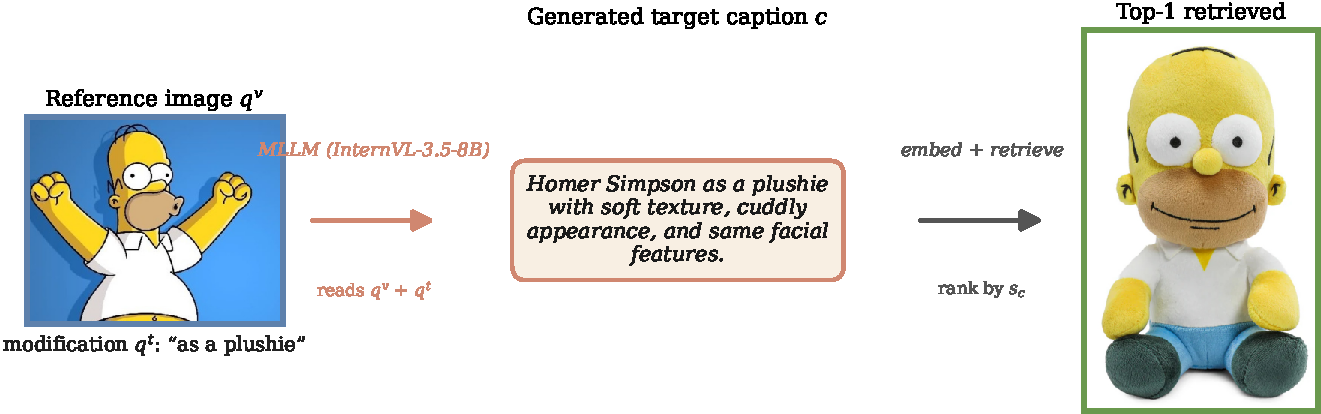
\includegraphics[width=\textwidth]{figures/caption_example.png}
\caption[Example of target-caption generation.]{Given the reference image and
the modification text, the MLLM generates a description of the intended target
image, which is then embedded and used as a third retrieval signal.
\label{fig:caption_example}}
\end{figure}

\begin{table}[h!]
\centering
\begin{tabular}{l l}
\toprule
ID & Instruction (summary) \\ \midrule
1\_8b   & shared core; full instance-focused rules \\
2\_8b   & core + explicit identifiable-name handling / generic fallback \\
3\_8b   & core; one-paragraph caption; stricter naming rule \\
4\_8b   & core + removes incidental original-image details (more general) \\
5\_8b   & two-stage: identify instance, then apply modification \\
6\_A\_8b & two-caption variant, A = more informative (best single) \\
6\_B\_8b & two-caption variant, B = short, instance + modification only \\
7\_8b   & two-stage + preserves explicit visual identifiers \\
8\_8b   & atomic-constraint decomposition + coverage + self-check \\
\bottomrule
\end{tabular}
\caption[Caption-generation instruction variants.]{The nine instruction
variants used to prompt the MLLM. \texttt{avg-9} averages the text embeddings of
all nine (Equation~\eqref{eq:avg9}); the verbatim prompts are reproduced in
Appendix~\ref{...}.\label{tab:instructions}}
% HIGHLIGHT: decide whether to include the verbatim prompts as an appendix.
% The full text is in artifacts/caption_files_Amin/prompts/internvl_instructions.md
\end{table}

% =====================================================================
\section{Triplet Late-Fusion Scoring}\label{sect:method_fusion}
% =====================================================================

The three branches of Section~\ref{sect:method_overview} produce, for a query
$q = (\qv, \qt)$ with generated caption $\qc$ and a candidate database image
$\xdb$, the three cosine similarities
\begin{align}
  \sv &= \simop\!\big(\encv(\qv),\, \encv(\xdb)\big), \label{eq:s_img}\\
  \st &= \simop\!\big(\enct(\qt),\, \encv(\xdb)\big), \label{eq:s_txt}\\
  \sc &= \simop\!\big(\enct(\qc),\, \encv(\xdb)\big). \label{eq:s_cap}
\end{align}
We fuse them by the \emph{clamped triplet product}
\begin{equation}\label{eq:triplet}
    s_{\text{triplet}}(q, \xdb) =
    \clamp\!\big(\sc\big)\cdot
    \clamp\!\big(\st\big)\cdot
    \clamp\!\big(\sv\big),
    \qquad
    \clamp(s) = \max(s, 0),
\end{equation}
and rank the database by $s_{\text{triplet}}$.

\paragraph{Why a product.} The product behaves as a soft logical
\textsc{and}: a candidate scores highly only if it agrees with \emph{all three}
signals -- it must look like the same instance ($\sv$), be consistent with the
modification text ($\st$), and match the imagined-target description ($\sc$). A
candidate that satisfies only one or two terms is heavily down-weighted, which
is exactly the behaviour needed against the instance-level hard negatives of
Section~\ref{sect:method_problem}: visual negatives fail $\st$ and $\sc$, while
textual negatives fail $\sv$. A sum, by contrast, would let one strong term mask
the failure of another and would reward the very hard negatives the benchmark is
designed around.

\paragraph{Why clamping.} Cosine similarities can be negative. Without
clamping, the product of two negative terms would become a large positive score
-- spuriously promoting candidates that are \emph{dissimilar} on two branches --
and a single negative term could flip the sign of the whole score. Clamping each
similarity to $[0, \infty)$ before multiplying removes these sign artefacts and
keeps the product monotone in each branch.

\paragraph{Relation to the duplet baseline.} Dropping the caption term recovers
the duplet baseline of Equation~\eqref{eq:duplet}. The triplet score is thus a
strict, additive extension of \textsc{Basic}'s fusion by the proposed third
modality; Chapter~\ref{chapt:results} measures the gain this term provides.

% =====================================================================
\section{Implementation Details}\label{sect:method_impl}
% =====================================================================

\paragraph{Software and hardware.} The pipeline is implemented in Python with
PyTorch. Contrastive backbones are loaded through OpenCLIP and HuggingFace
Transformers, and the InternVL caption generator runs through HuggingFace
Transformers. All large-scale embedding and retrieval jobs run on a SLURM-managed
HPC cluster with NVIDIA GPUs (A5000 and A100 nodes).
% HIGHLIGHT: state the exact GPUs/driver/CUDA you want on record, and the
% library versions (openclip, transformers, torch) for reproducibility.

\paragraph{Caption generation settings.} Captions are generated with
InternVL-3.5-8B using its high-resolution tiling input and a fixed decoding
configuration shared across all nine instructions.
% HIGHLIGHT: fill in the EXACT InternVL-8B generation settings you used
% (temperature, max new tokens, number of tiles). The 4B REPL used
% temp=0.7 / 12 tiles / 512 tokens -- confirm the 8B batch run matches.

\paragraph{Embedding the full database.} Embedding the full $752$K-image
database is the most expensive step. It is performed once per backbone in a
\emph{sharded, checkpointed} manner: the database is split into shards, each
shard is embedded independently and written to disk, and a job that is preempted
or fails resumes from the last completed shard. Query images, query texts,
captions, and the contextualized-text corpora are embedded the same way.
Embeddings are cached on disk and reused across all retrieval configurations, so
that the expensive encoding is never repeated when only the fusion or
post-processing changes.

\paragraph{Development subset.} To iterate quickly, ablations are run on a fixed
$20\%$ instance subset (\texttt{instance\_sample20\_seed42}: $400$ queries and
$143{,}769$ database images). The subset is sampled by instance with a fixed
seed so that it is reproducible and representative. We treat it as a fair
development proxy because the subset duplet baseline closely matches the full
baseline (the CLIP-L text$\times$image macro-mAP is within a fraction of a point
of the paper's full-dataset baseline), so trends observed on the subset are
expected to hold at full scale; the headline numbers in Chapter~\ref{chapt:results}
are nonetheless always reported on the full dataset.

\paragraph{Result storage and reproducibility.} Retrieval rankings and the
associated evaluation artefacts are stored in a compact, sparse (CSR-packed)
format, alongside the configuration that produced them. All runs are driven by
explicit configuration files and fixed random seeds, so that every reported
number can be regenerated from the stored embeddings and configs.
